
\documentclass[12pt,titlepage]{article}
%\renewcommand{\baselinestretch}{1} 
%\linespread{0.828}
%\usepackage{setspace}
%\singlespacing
%\onehalfspacing
%\doublespacing
\usepackage[pdftex]{color,graphicx}
%\usepackage{polski}
\usepackage{geometry}
\geometry{a4paper, margin=2cm}
%\usepackage{indentfirst}
\usepackage{listings}
\usepackage{url}
\usepackage{rotating}
\usepackage{booktabs}
\usepackage[super]{nth}
%\usepackage{multirow}
%\usepackage{cite}
%\usepackage{float}
%\usepackage{amsmath}
%\usepackage{amstext}
%\usepackage{ amssymb }
%\usepackage[toc,page]{appendix}
%\usepackage{ragged2e}
%\usepackage{epstopdf}
%\usepackage{epsfig}
%Jesli uzywasz kodowania polskich znakow ISO-8859-2 nastepna linia powinna byc 
%odkomentowana
\usepackage[latin2]{inputenc}
%\usepackage{relsize}
%\usepackage{minted}
%\def\textsubscript#1{\ensuremath{_{\mbox{\textscale{.6}{#1}}}}}
\usepackage{pdflscape}
\usepackage{multirow}
%\usepackage{etoolbox}
%\patchcmd\thebibliography
% {\labelsep}
% {\labelsep\itemsep=0pt\relax}
% {}
% {\typeout{Couldn't patch the command}}
\setcounter{tocdepth}{1}
%\usepackage[linktoc=all]{hyperref}
\usepackage{hyperref}
\hypersetup{hidelinks,linktocpage,linktoc=all}


\usepackage{fancyhdr}
\renewcommand{\footrulewidth}{0.4pt}% default is 0pt
\pagestyle{fancy}
\lfoot{WM-I-S2-E3-IDG}
\lhead{}
\rfoot{\thepage}
\cfoot{Information Persistence in Dynamic Graphs}


\title{Interconnection: from Dynamic Graphs to Social Networks\\
	\vspace{20pt}
\textbf{Project: Information Persistence in Dynamic Graphs}}
\author{Anna Kelm, Piotr Plebanski\\
	110455, 121309
} 

% Tu jest dobre miejsce na Twoje w�asne makra i~�rodowiska:
%\newtheorem{defi}{Definicja}[section]
%\pagenumbering{gobble}% Remove page numbers (and reset to 1)
% koniec definicji

\usepackage{minted}
\setminted{autogobble, breaklines, breakanywhere}

\newminted[bash]{console}{formatcom=\AWP, autogobble, breaklines, breakanywhere, xrightmargin=90pt,xleftmargin=-6pt}
\newminted[bashSamba]{console}{formatcom=\ASamba, autogobble, escapeinside=;;, breaklines, breakanywhere, xrightmargin=90pt,xleftmargin=-6pt}
\newminted[bashMysql]{console}{formatcom=\AMysql, autogobble, escapeinside=;;, breaklines, breakanywhere, xrightmargin=90pt,xleftmargin=-6pt}
\newminted[bashMdb]{console}{formatcom=\Mdb, autogobble, breaklines, breakanywhere, xrightmargin=90pt,xleftmargin=-6pt}

\newminted[bashR1]{console}{formatcom=\AR, autogobble, escapeinside=;;, breaklines, breakanywhere, xrightmargin=90pt,xleftmargin=-6pt}
\newminted[mysq]{mysql}{formatcom=\AMysql, autogobble, escapeinside=;;, breaklines, breakanywhere, xrightmargin=90pt,xleftmargin=-6pt}
\newminted[bashScript]{bash}{autogobble, breaklines, breakanywhere}

% ------------------------------------------------------
\usepackage[framemethod=TikZ]{mdframed}

\surroundwithmdframed[linewidth=0.5pt, backgroundcolor=gray, roundcorner=5pt, innerbottommargin=2pt, innertopmargin=3pt]{bash}
\surroundwithmdframed[linewidth=0.5pt, backgroundcolor=gray]{bashScript}



\newcommand{\User}{%
	\def\FancyVerbFormatLine##1{\$\,##1}%
}

\newcommand{\Root}{%
	\def\FancyVerbFormatLine##1{\#\,##1}%
}

\newcommand{\AS}{%
	\def\FancyVerbFormatLine##1{[ania@s1]\$\,##1}%
}

\newcommand{\ASamba}{%
	\def\FancyVerbFormatLine##1{[ania@sambapss]\$\,##1}%
}

\newcommand{\AMysql}{%
	\def\FancyVerbFormatLine##1{mysql$>$\,##1}%
}

\newcommand{\Mdb}{%
	\def\FancyVerbFormatLine##1{MariaDB [(none)]>\,##1}%
}

\newcommand{\AR}{%
	\def\FancyVerbFormatLine##1{\$\,##1}%
}

\newcommand{\AWP}{%
	\def\FancyVerbFormatLine##1{[kajack@wpr]\$\,##1}%
}

\newcommand{\AT}{%
	\def\FancyVerbFormatLine##1{[ania@thinkcentre]\$\,##1}%
}

\lstdefinestyle{DOS}
{
	backgroundcolor=\color{black},
	basicstyle=\scriptsize\color{white}\ttfamily,
	breaklines=true,
}

\definecolor{gray}{rgb}{0.98,0.98,0.98}
\definecolor{LightYellow}{RGB}{255,255,240}
\lstdefinestyle{PLIK}
{
	basicstyle=\footnotesize\ttfamily,
	breaklines=true,
	backgroundcolor=\color{LightYellow},
	 frame=leftline
}
% \newcommand\shellthree[1]{\colorbox{blue}{\parbox[t]{\textwidth}{\lstinline[style=PLIK,mathescape]`#1`}}}

\lstdefinestyle{OUTPUT}
{
	basicstyle=\small\ttfamily,
	breaklines=true
}





\begin{document}

\maketitle
\setcounter{tocdepth}{2}
\tableofcontents

\clearpage
\section{Introduction}
This project aims at investigation the conditions influencing the information persistance within a dynamic graph. Three dynamic graph models were selected: Edge Markovian, Random Waypoint (RWP) and Manhattan model. While a set of nodes in each graph remained constant, the set of edges evolved according to the graph model which influenced the transmission of the information with a fixed lifetime.



\section{Experimental}

\subsection{Graph parameter ranges}
Environment settings and parameter ranges common for all models:
\begin{itemize}
	\item number of experiments repetitions: 15
	\item maximum number of iterations: 1000
	\item environment size: 1000x1000
	\item number of nodes, n:  \{50, 100, 200, 300\}
\end{itemize}
Parameters for geometric graph models (Manhattan and RWP)
\begin{itemize}
	\item distance threshold, d: \{20, 30, 50, 70, 80, 100, 120\}
\end{itemize}
Parameters for Manhattan model:
\begin{itemize}
	\item number of parallel streets is in each direction: 10
\end{itemize}
Parameters for Edge Markovian model:
\begin{itemize}
	\item parameters for Edge Markovian model, $p$ and $q$, are probabilities of nodes staying connected or unconnected, respectively, as shown in Fig~\ref{fig:markovian}. A $p + q = 1$, this Edge Markovian model corresponds to Erdos-Renyi graph model. The selected values of parameters p correspond to mean graph density in RWP model with distance threshold d (also knows as excluded volume). That is:\cite{Dall2002}:
	\begin{equation}
	p_i = \frac{4\pi\cdot d_i^2}{l^2}
	\end{equation}
	where l=1000 denotes the size of the environment. Calculated values of $p_i$ are \{ 0.001, 0.003, 0.008, 0.0015, 0.02, 0.031, 0.045 \}.
	
\end{itemize}

\begin{figure}
	\centering
	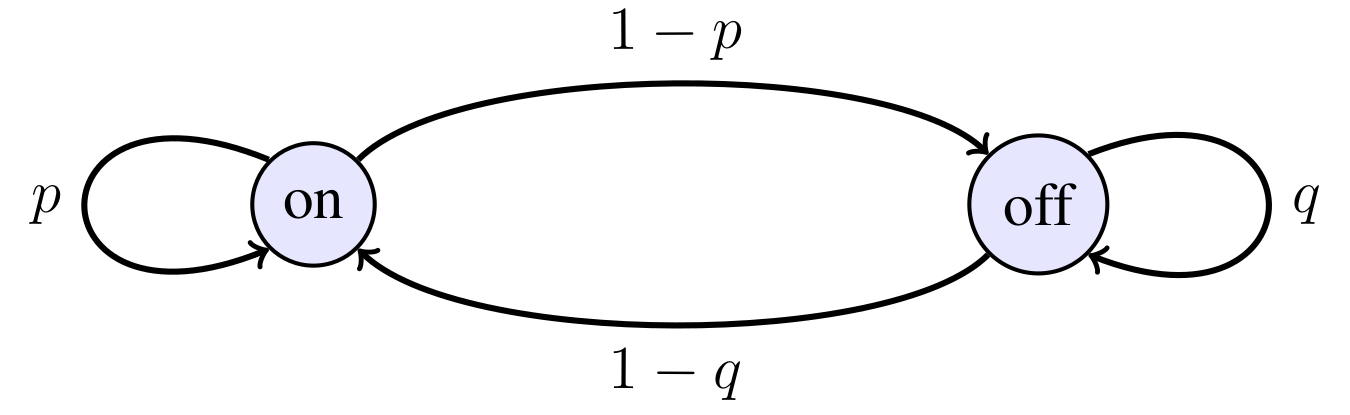
\includegraphics[width=0.7\linewidth]{screenshot008}
	\caption{Automata regulating the state of an edge in an edge-markovian dynamic graph.[source: project description by F. Guinand]}
	\label{fig:markovian}
\end{figure}



\subsection{The transmission of information}
In each graph, at the start of each experiment one was was provided with the information of a fixed time-to-live (TTL). The possible values of TTL were: \{1, 2, 3, 4, 5\} iterations. In each iteration, each node X with the information broadcasted it to the nodes $\{Y_i\}$ that had a common edge with X. If a node $\{Y_i\}$ does not have the information, it receives its copy with a full lifetime (equal to the starting lifetime). After every iteration, the current information TTLs in the nodes decrease by 1. A node with information TTL=0 does not carry the information. Each experiment was terminated when either the information was no longer present in the whole graph of the number of iterations reach 1000.


\subsection{Experimental procedure}
Experiments were performed with the use of GraphStream library\cite{Dutot2007}, version 1.3. While the graph simulation was performed in Java with GraphStream, the experiment parameter settings, collection of the results and plotting were performed in Python 3.10. The *.jar package containing the simulations was invoked from Python with the use of pyjnius Python library. The details of the experimental setup and source code can be found at: \url{github.com/akelm/interconnection_final_project}.


For each type of graph model, there were $4 \cdot 7 \cdot 5 = 140$ possible parameter settings and each experiment with given experimental settings was run 15 times for the statistics. In total, for all graphs, 6300 experiments were run.


Notably, it needs to be mentioned that experiments for Edge Markovian graph wre performed NOT with a GraphStream library, but with a simple representation of graph using connectivity matrix. The reason behind this decision was the poor speed of the simulation, most probably due high edge nervousness.


\subsection{Recorded graph characteristics}
Graph characteristics collected during experiments in each iteration:
\begin{itemize}
	\item number of edges,
	\item number of nodes with information,
	\item edge nervousness, defined as a Jaccard distance between node sets in $i$th and $i=1$ iterations,
	\item number of connected components.
\end{itemize}
Calculated after the experiments:
\begin{itemize}
	\item success rate at preserving information to the 1000th iteration.
\end{itemize}


\section{Results and Discussion}
\subsection{The graphs characteristics}
Fig~\ref{fig:density}-\ref{fig:nervousness} present the graphs characteristics in all three graph models for different $n$ and $d$/$p$, averaged over 15 repeated experiments. 


The graph density, as shown in Fig~\ref{fig:density}, is almost constant for the Edge-Markovian graph, while it changes by up to 100\% in the course of 1000 iterations. The graph density grows approximately quadratically with the distance threshold (or $p$ in Edge Markovian graph) and seems independent of the node density. However, the considerable noise in the graph density, decreasing with increasing n, seems to indicate higher the temporal graph density oscillations for lower number of nodes.

The number of connected components divided by $n$ (Fig~\ref{fig:connectedcomp}) spans from $1/n$ in the connected graph to $1$ for a graph with 0 edges. This measure is in a close relationship with graph density -- the denser the graph, the lower number of connected components it owns. Contrary to the graph density, the number of connected components (divided by n) depends also on $n$ -- it decreases with $n$.  


Fig~\ref{fig:nervousness} shows the time traces of edge nervousness in all three graph models for different $n$ and $d$ or $p$. Edge nervousness is very high in Edge Markovian graph and close to 0 for geometric graph models. This probably originates from the fact, that in an Edge Markovian graphs, edges disappear stochastically with high probability -- meaning that the edge formed in $i-1$th iteration will almost certainly disappear in the $i$th iteration. Meanwhile, in geometric graphs, nodes need to move away from each other in order to for the edge to be removed, which takes more time. In all graph models, the nervousness lowers with $d$/$p$ and is very noisy in graph with low $n$.



\begin{sidewaysfigure}[!h]
	\centering
	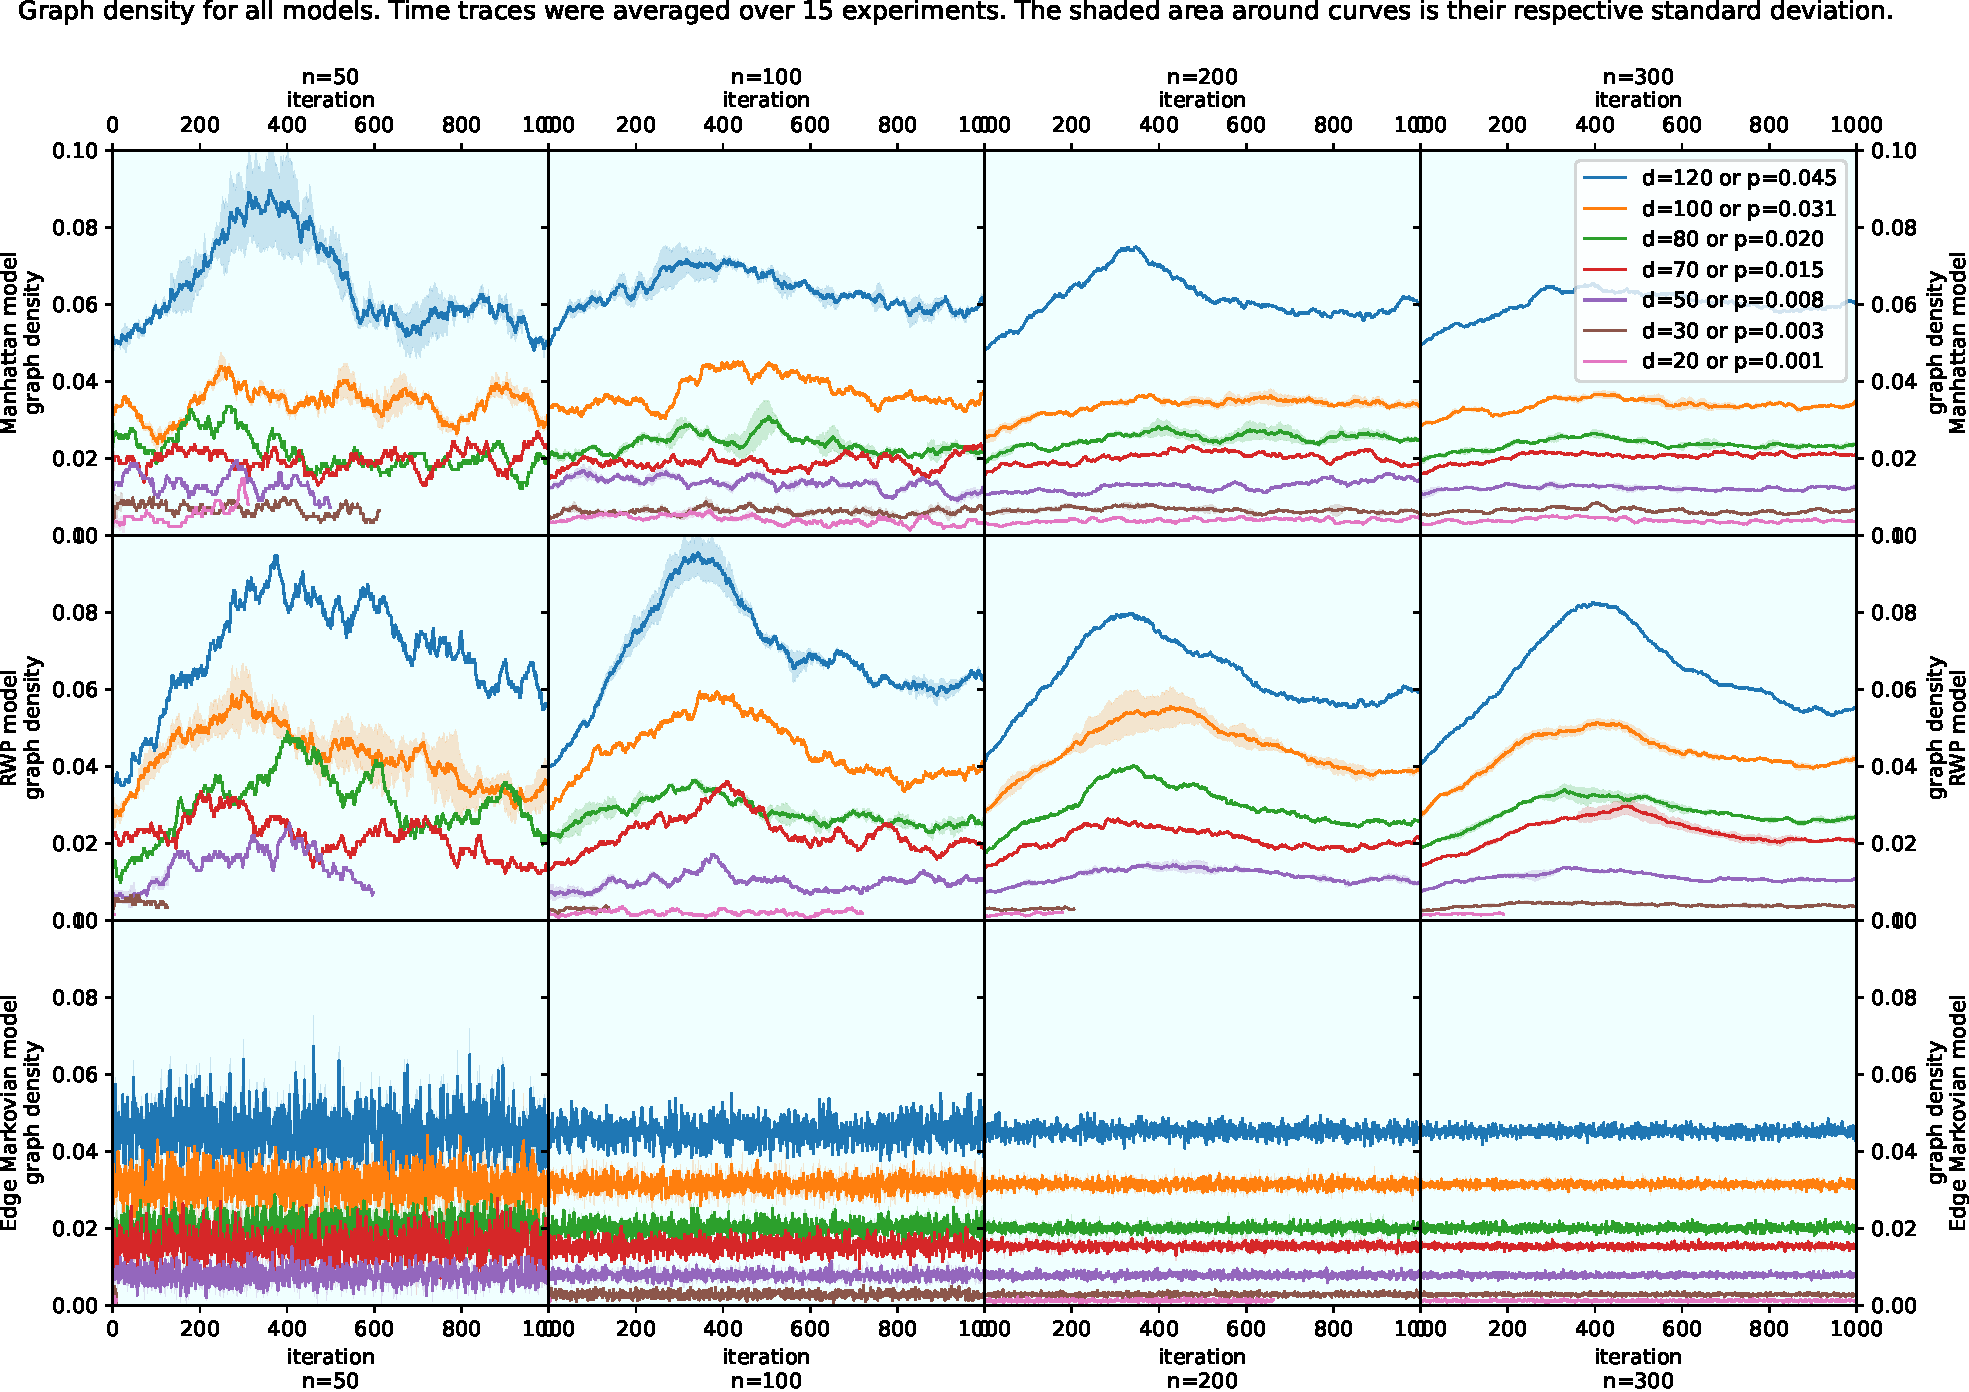
\includegraphics[width=1\linewidth]{results/density}
	\caption{Graph density for all models. Time traces were averaged over 15 experiments. The shaded area around curves is their respective standard deviation.}
	\label{fig:density}
\end{sidewaysfigure}
\begin{sidewaysfigure}[!h]
	\centering
	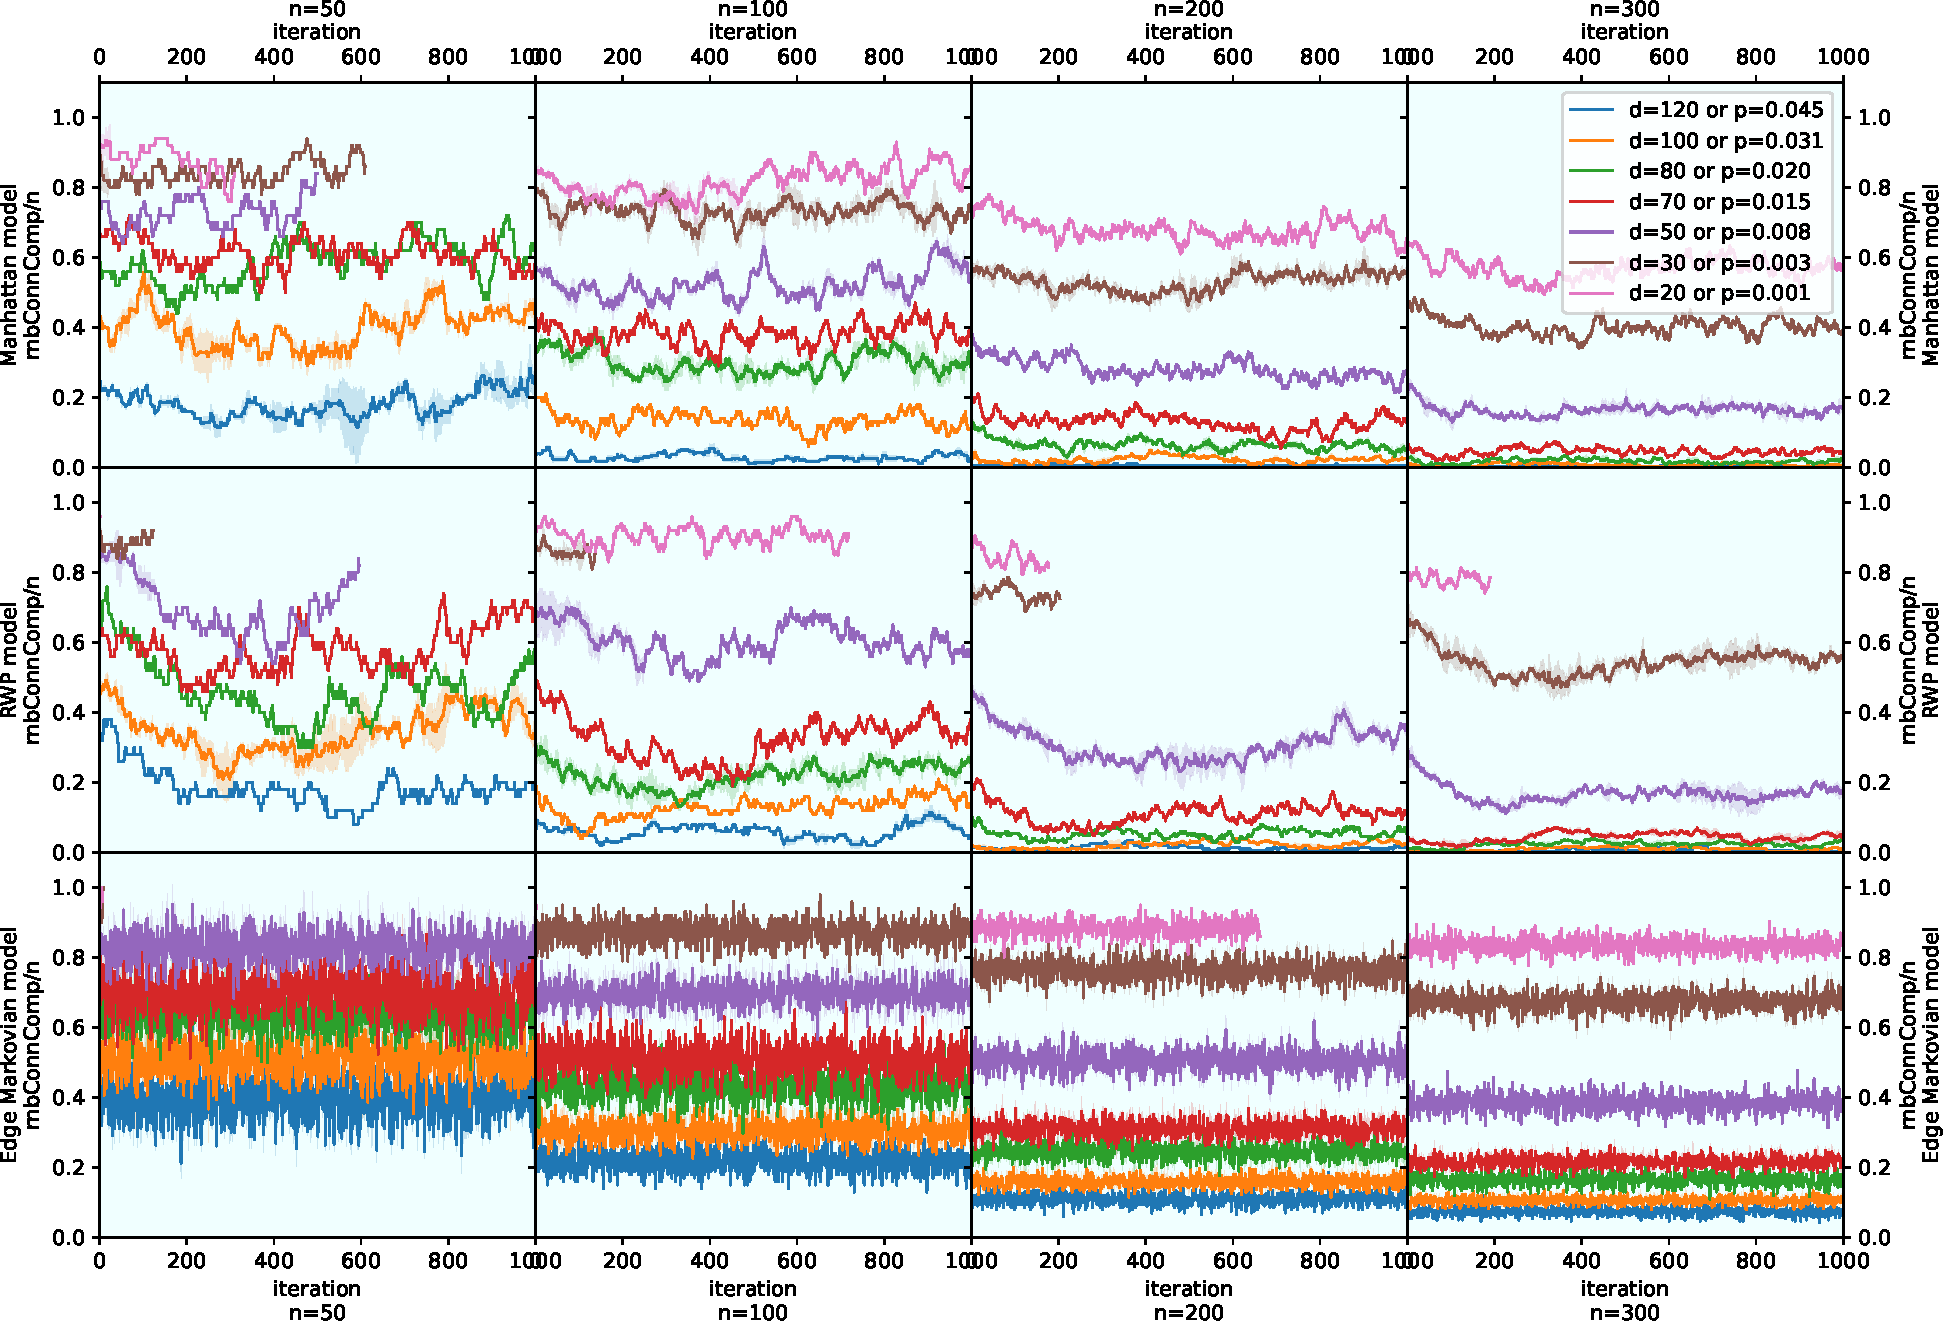
\includegraphics[width=1\linewidth]{results/connected_comp}
	\caption{Number of connected components normalized to the number of nodes for all models. Time traces were averaged over 15 experiments. The shaded area around curves is their respective standard deviation.}
	\label{fig:connectedcomp}
\end{sidewaysfigure}
\begin{sidewaysfigure}[!h]
	\centering
	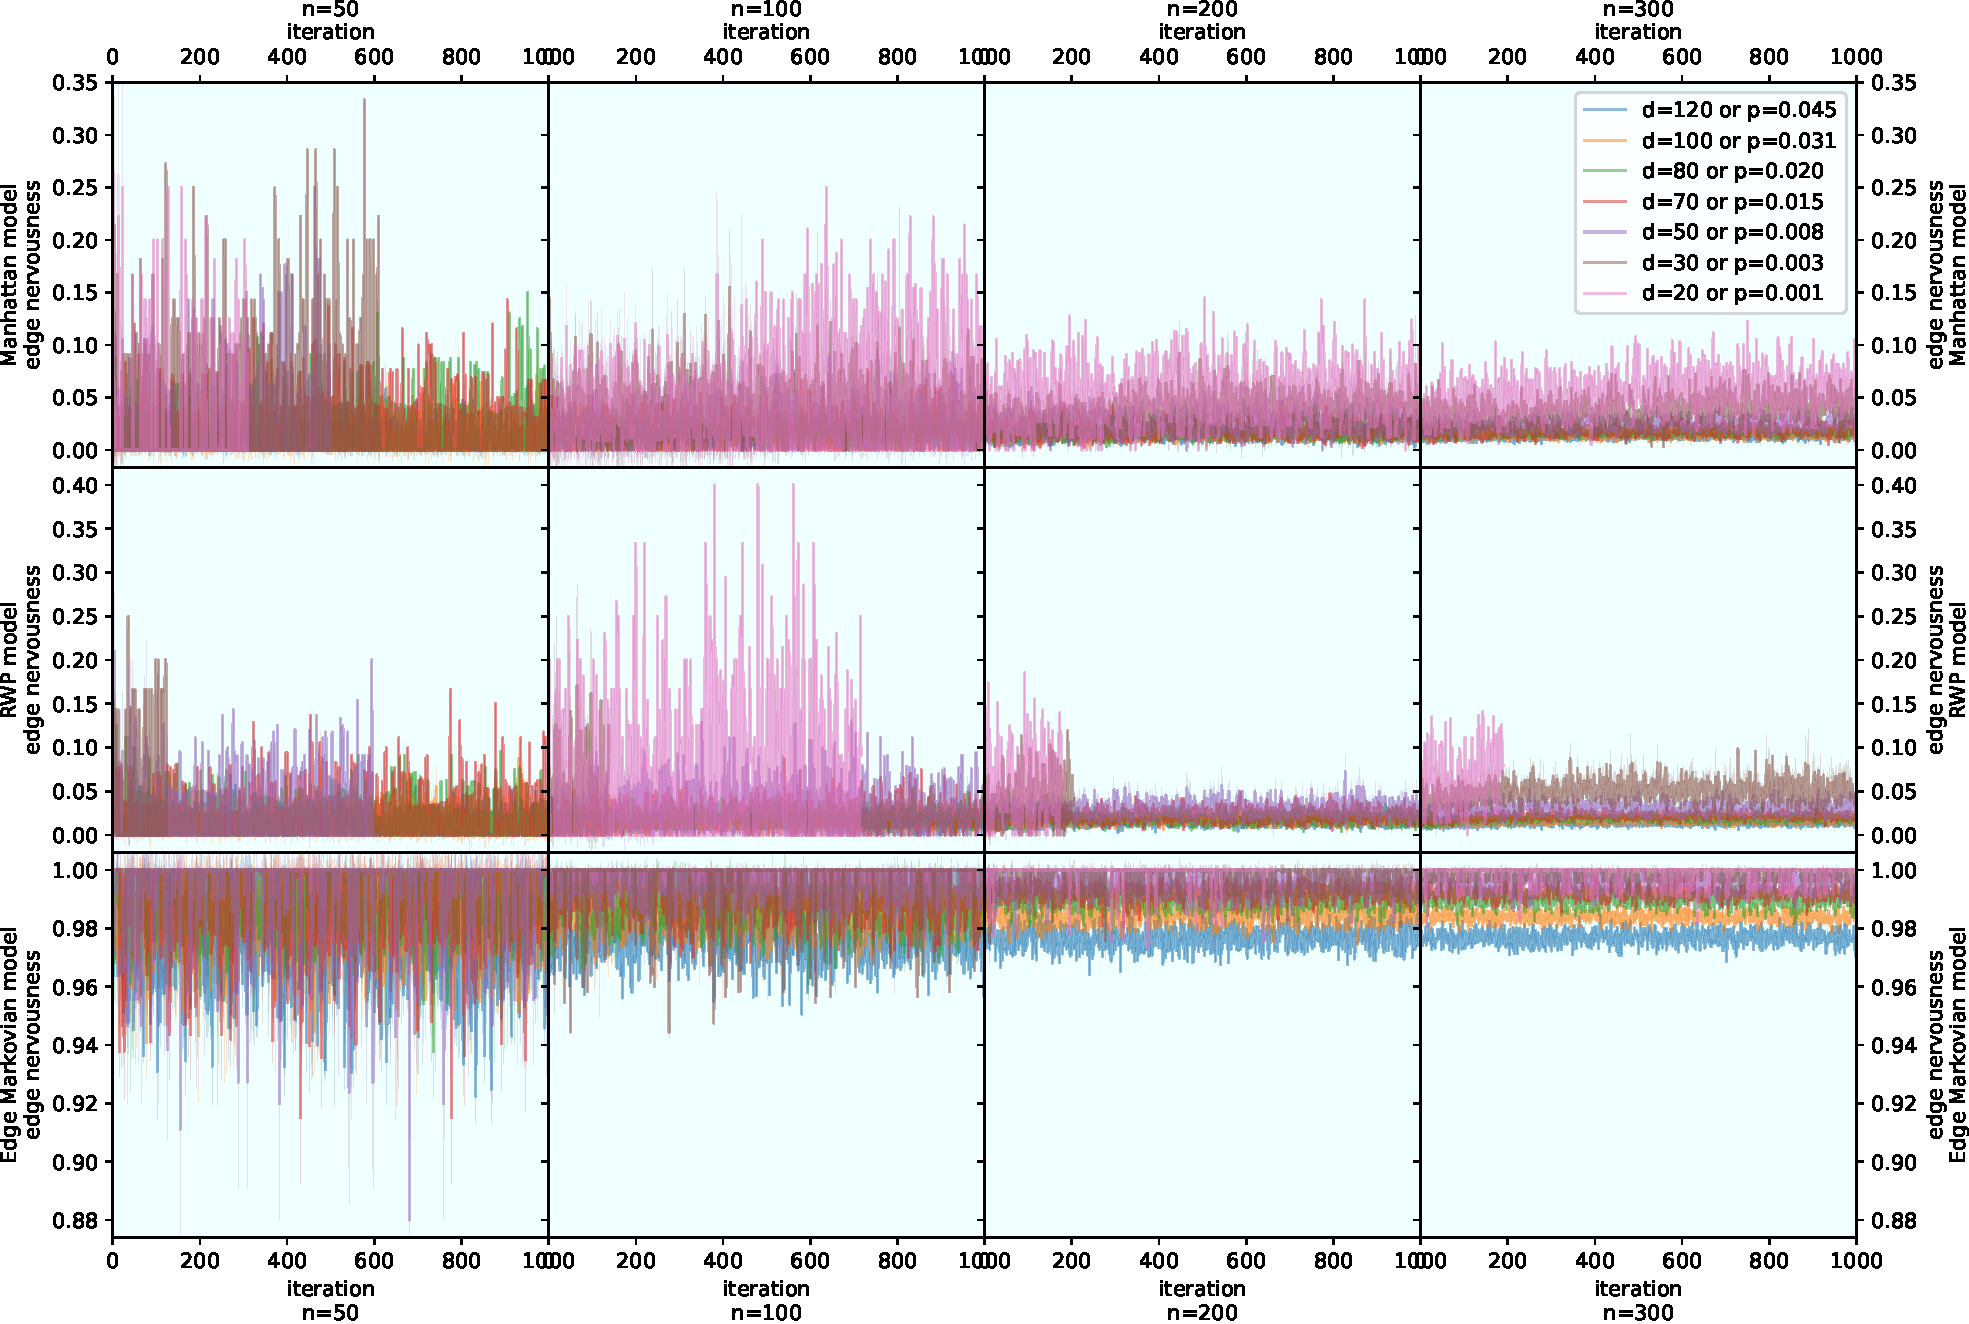
\includegraphics[width=\linewidth]{results/nervousness}
	\caption{Edge nervousness for all models. Time traces were averaged over 15 experiments. The shaded area around curves is their respective standard deviation.}
	\label{fig:nervousness}
\end{sidewaysfigure}



\subsection{The propagation and persistence of information}

In all of the expriments, the fraction of nodes with information in the Edge Markovian model (Fig~\ref{fig:fracinfoedge}) grows rapidly in $\leq 50$ iterations, after it reaches an equlibrium value which stays constant (modulo some noise) until the \nth{100} iterations. If the equilibrium value is comparable or lower to its temporal variations, the information has a high chance to be lost due to the high probability of the fraction of nodes with information reaching 0. These short-term temporal variations in Edge Markovian graph are considerably stronger that in the case of geometric graph, most probably due to very high nervousness. Reaching the equilibrium value of faction of nodes with information means that equal number of nodes loses and gains information. The values of equilibrium fraction of nodes with information, $p_{info}$ can be estimated by balancing the probability of receiving information by a node:
\begin{equation}
p_{rec} = (1-p_{info}) \cdot (1 - (1 - p +p\cdot(1-p_{info})   )^{n-1}  ) \approx (1-p_{info}) \cdot p \cdot p_{info} \cdot (n-1)
\end{equation}
with a probability that a node looses the information:
\begin{equation}
	p_{loss} = p_{info}/TTL
\end{equation}
which gives:
\begin{equation}\label{eqn:markovian}
	p_{info} = \frac{TTL \cdot p\cdot (n-1) - 1}{TTL \cdot p \cdot (n-1)}
\end{equation}
The plot of the values (Fig~\ref{fig:simulatedfracinfo}) calculated the aforementioned way yields values close to those obtained in the experiments, further supporting the explanations above.

\begin{figure}[H]
	\centering
	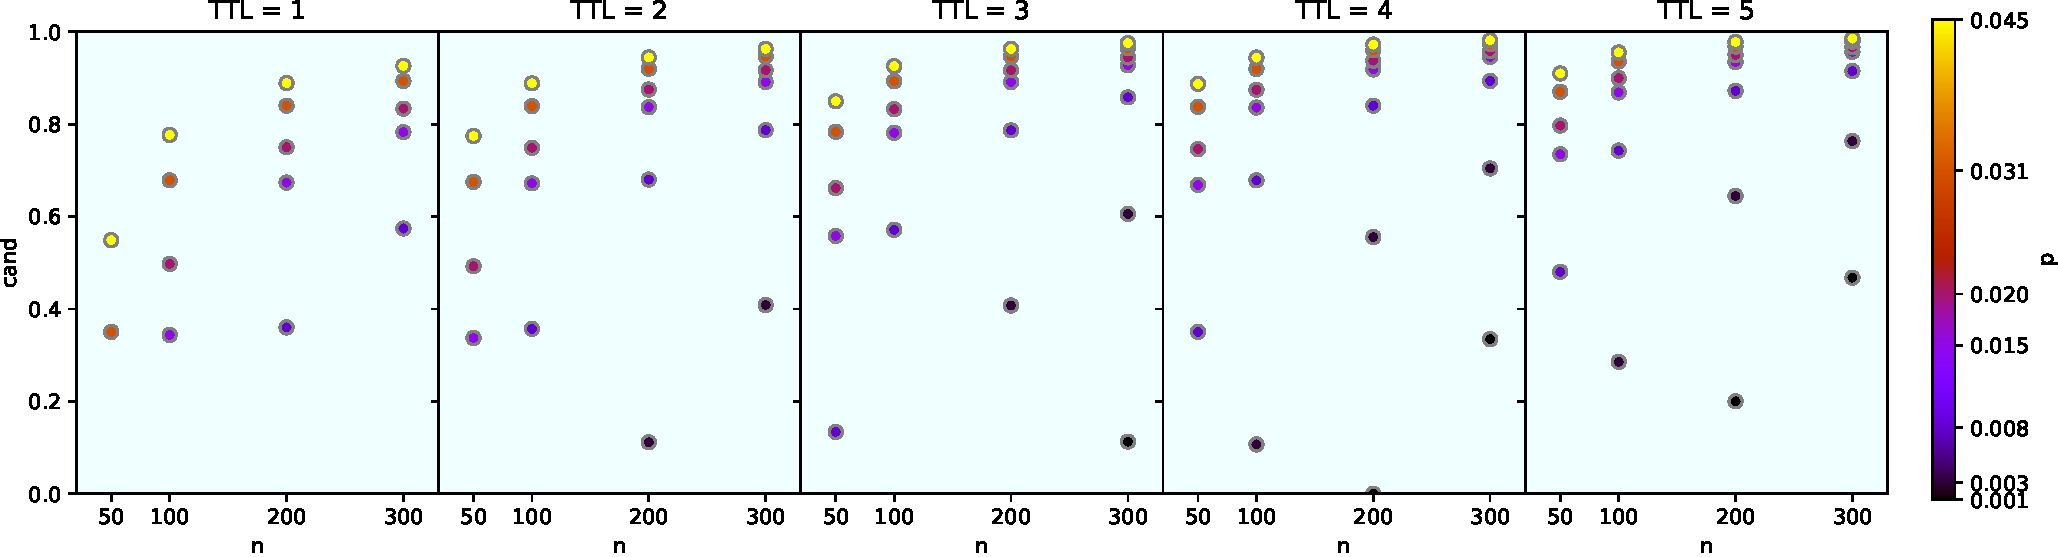
\includegraphics[width=1\linewidth]{simulated_frac_info}
	\caption{Fraction of the nodes with information for Edge Markovian graph estimated using Eq~\ref{eqn:markovian}.}
	\label{fig:simulatedfracinfo}
\end{figure}

In the case of the geometric graphs (Fig~\ref{fig:fracinfoman}-\ref{fig:fracinforwp}), such equilibrium value of nodes with information cannot be clearly observed at the same extent, however one can clearly see plateaus in fraction of nodes with information after much longer (approx. 200-500 iterations) rising phase. The values in the plateaus fluctuate over time due especially for low $n$ due to evolving in time uneven random surface node density in the graph, which controls the edges creation and destruction. It it also the origin of low edge nervousness, and low edge nervousness explains the slower spread of the information in comparison to Edge Markovian graph model. Furthermore, contrary to Edge Markovian graph model, the results clearly depict the correlation of the fraction of nodes with information rising time with the distance threshold (negative correlation) and the number of nodes (positive correlation). 

The Manhattan graph model (\ref{fig:fracinfoman}) has significant higher information fraction rising times for low $d$ values (20, 30, 50) compared to RWP model (\ref{fig:fracinforwp}). This probably is the results of a constraining the nodes movement to 10 streets in each direction, with the distance between neighboring streets of 100. Therefore for the $d$ values of 50 and lower, the nodes cannot form edges with nodes from a parallel streets and the transfer of information takes place with the help of nodes from perpendicular streets if the are close enough. $d$ higher than 50 makes the direct information transfer between the neighboring streets possible.


\begin{sidewaysfigure}[!h]
	\centering
	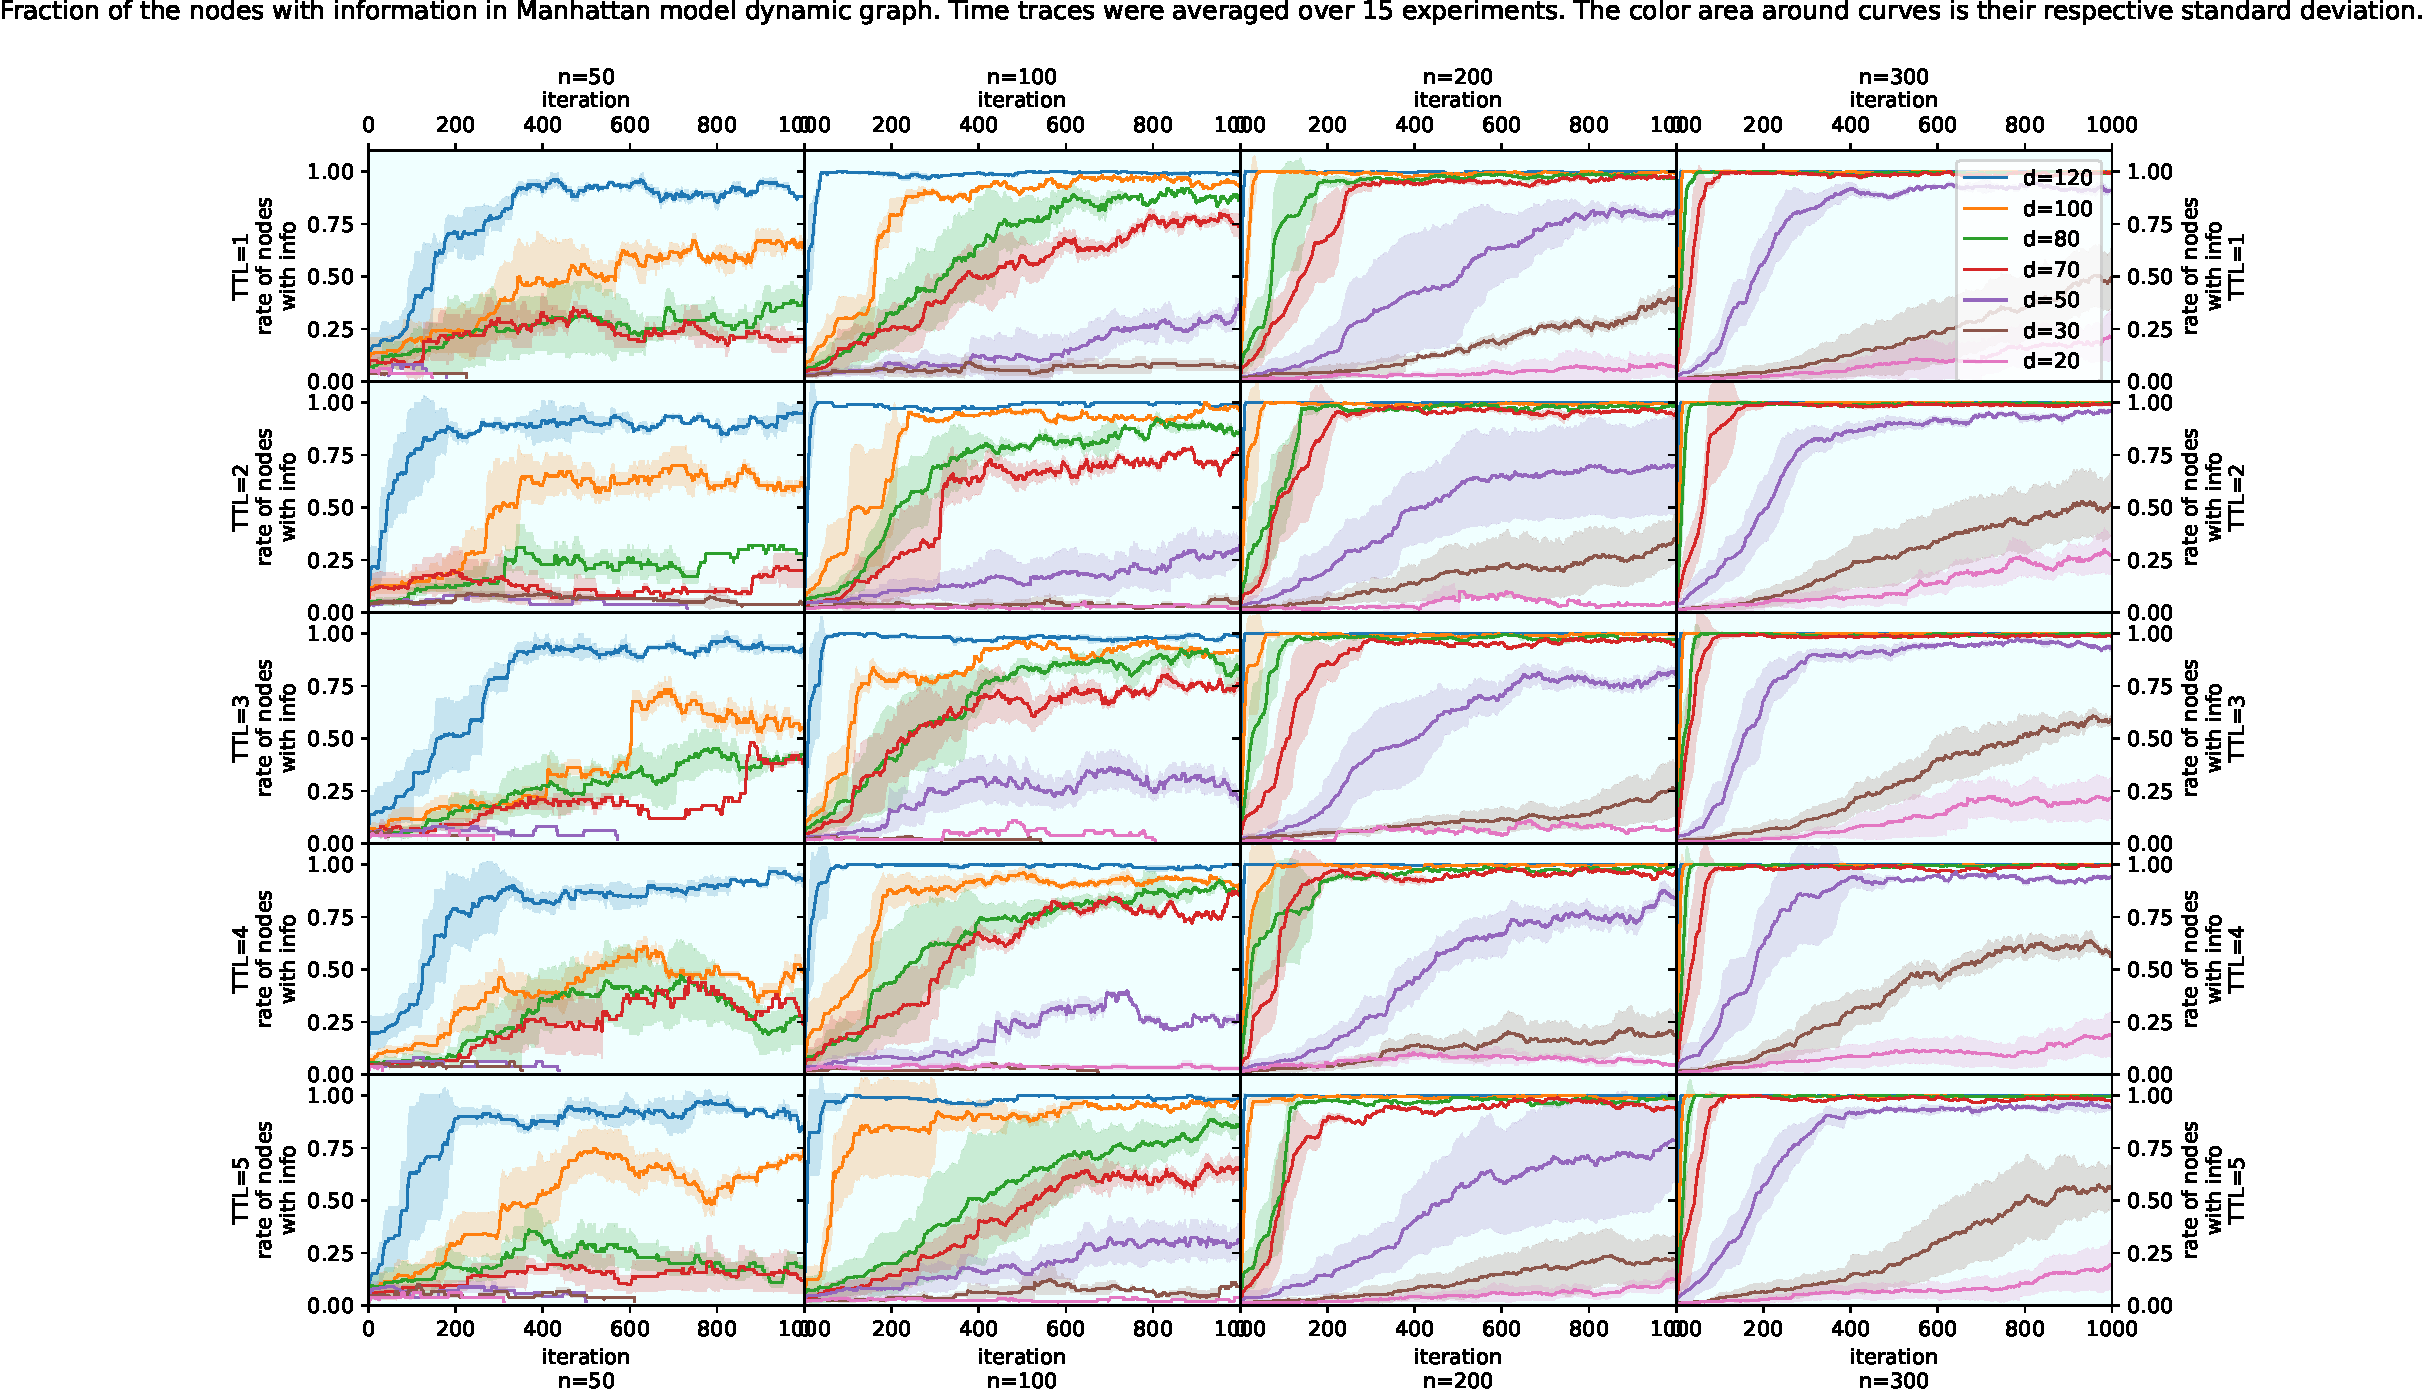
\includegraphics[width=1\linewidth]{results/frac_info_man}
	\caption{Fraction of the nodes with information in Manhattan model dynamic graph. Time traces were averaged over 15 experiments. The color area around curves is their respective standard deviation.}
	\label{fig:fracinfoman}
\end{sidewaysfigure}
\begin{sidewaysfigure}[!h]
	\centering
	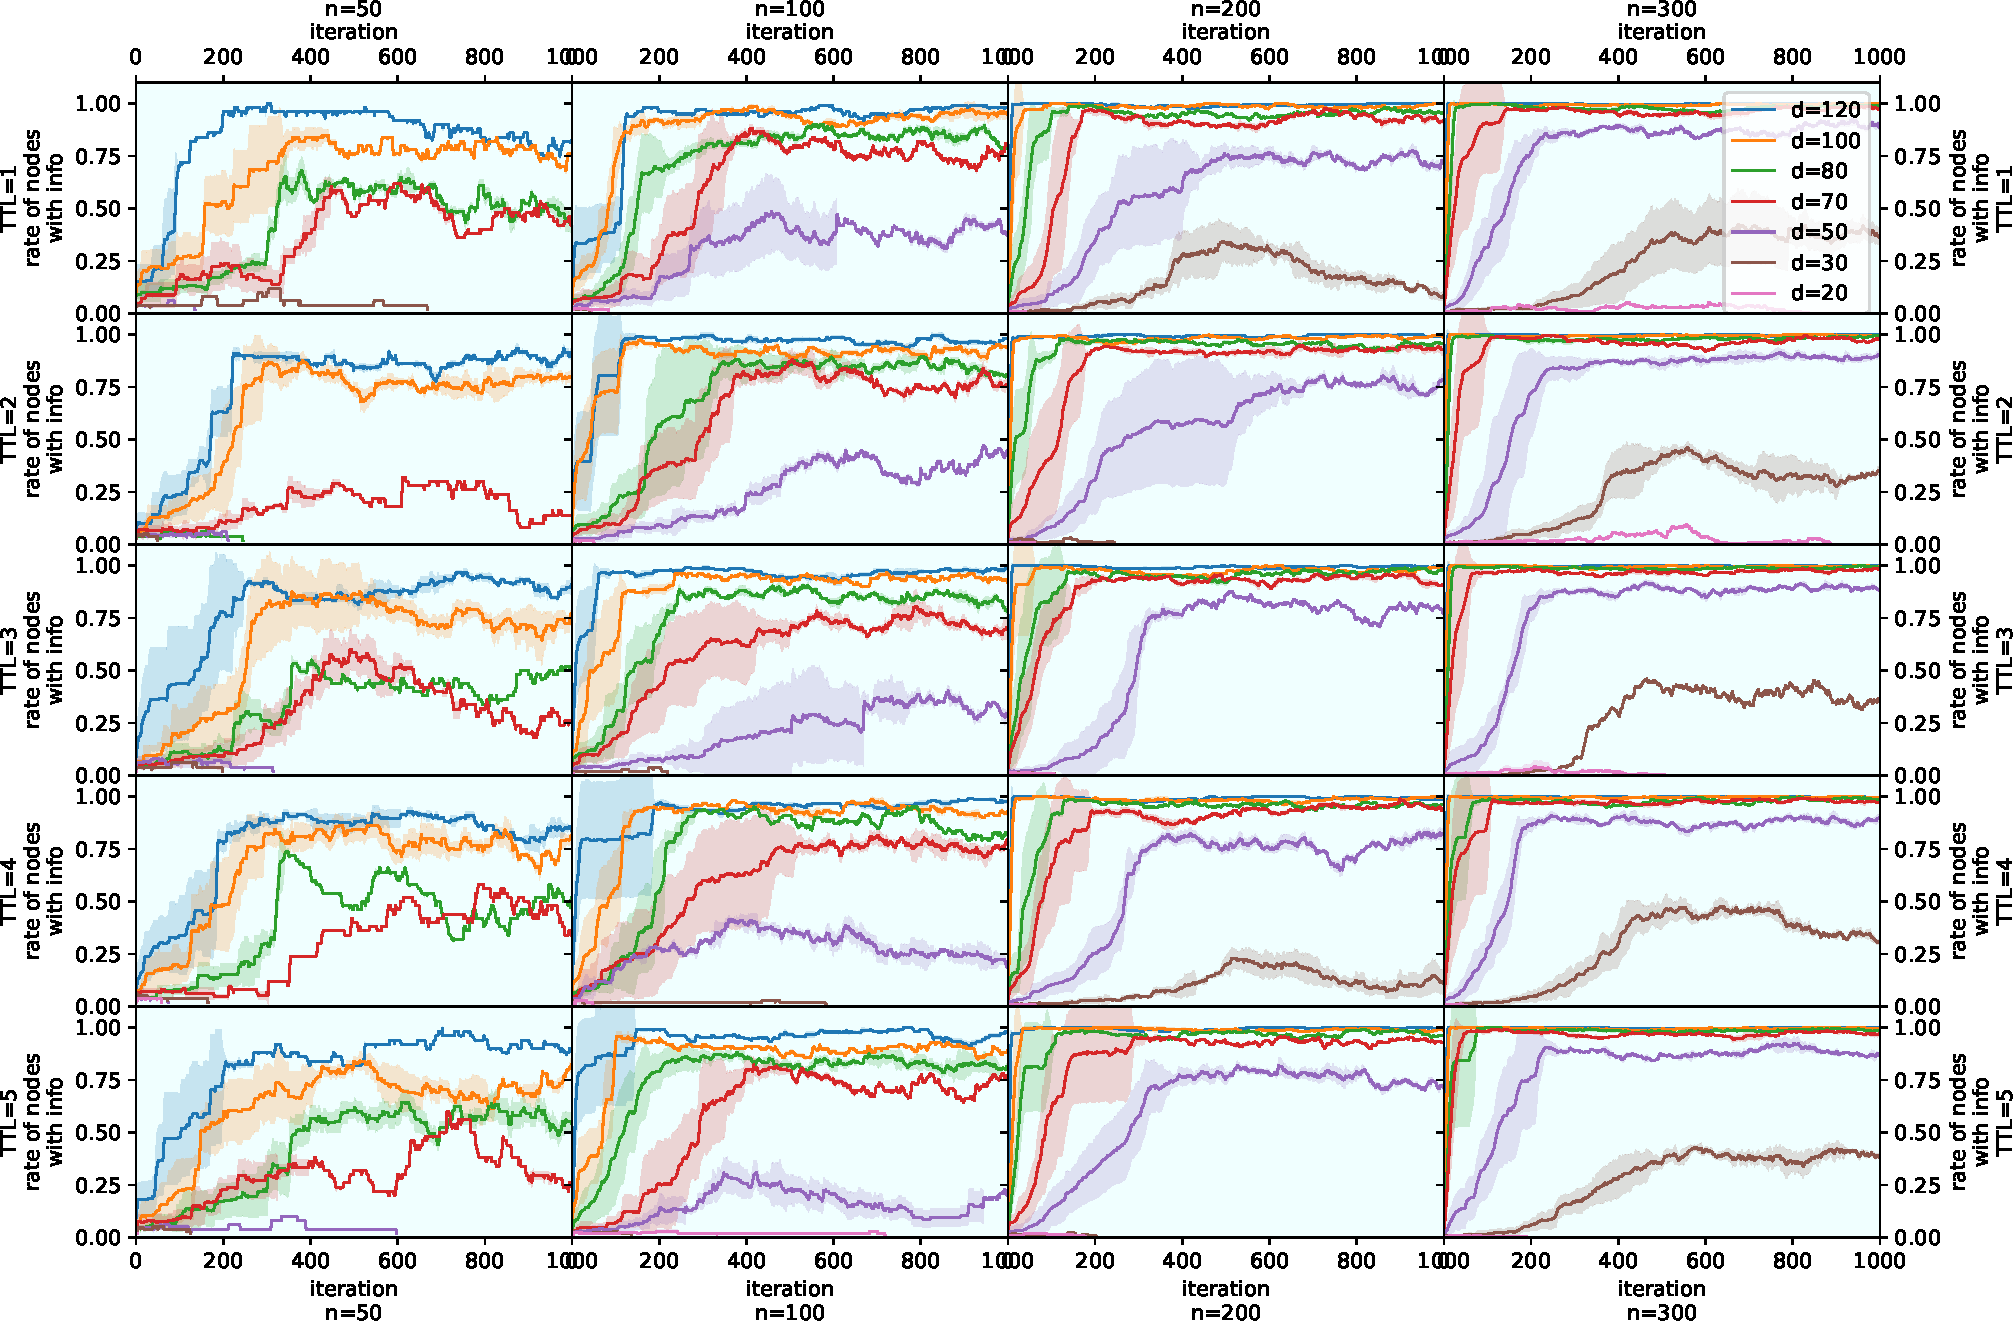
\includegraphics[width=1\linewidth]{results/frac_info_rwp}
	\caption{Fraction of the nodes with information in RWP model dynamic graph. Time traces were averaged over 15 experiments. The color area around curves is their respective standard deviation.}
	\label{fig:fracinforwp}
\end{sidewaysfigure}
\begin{sidewaysfigure}[!h]
	\centering
	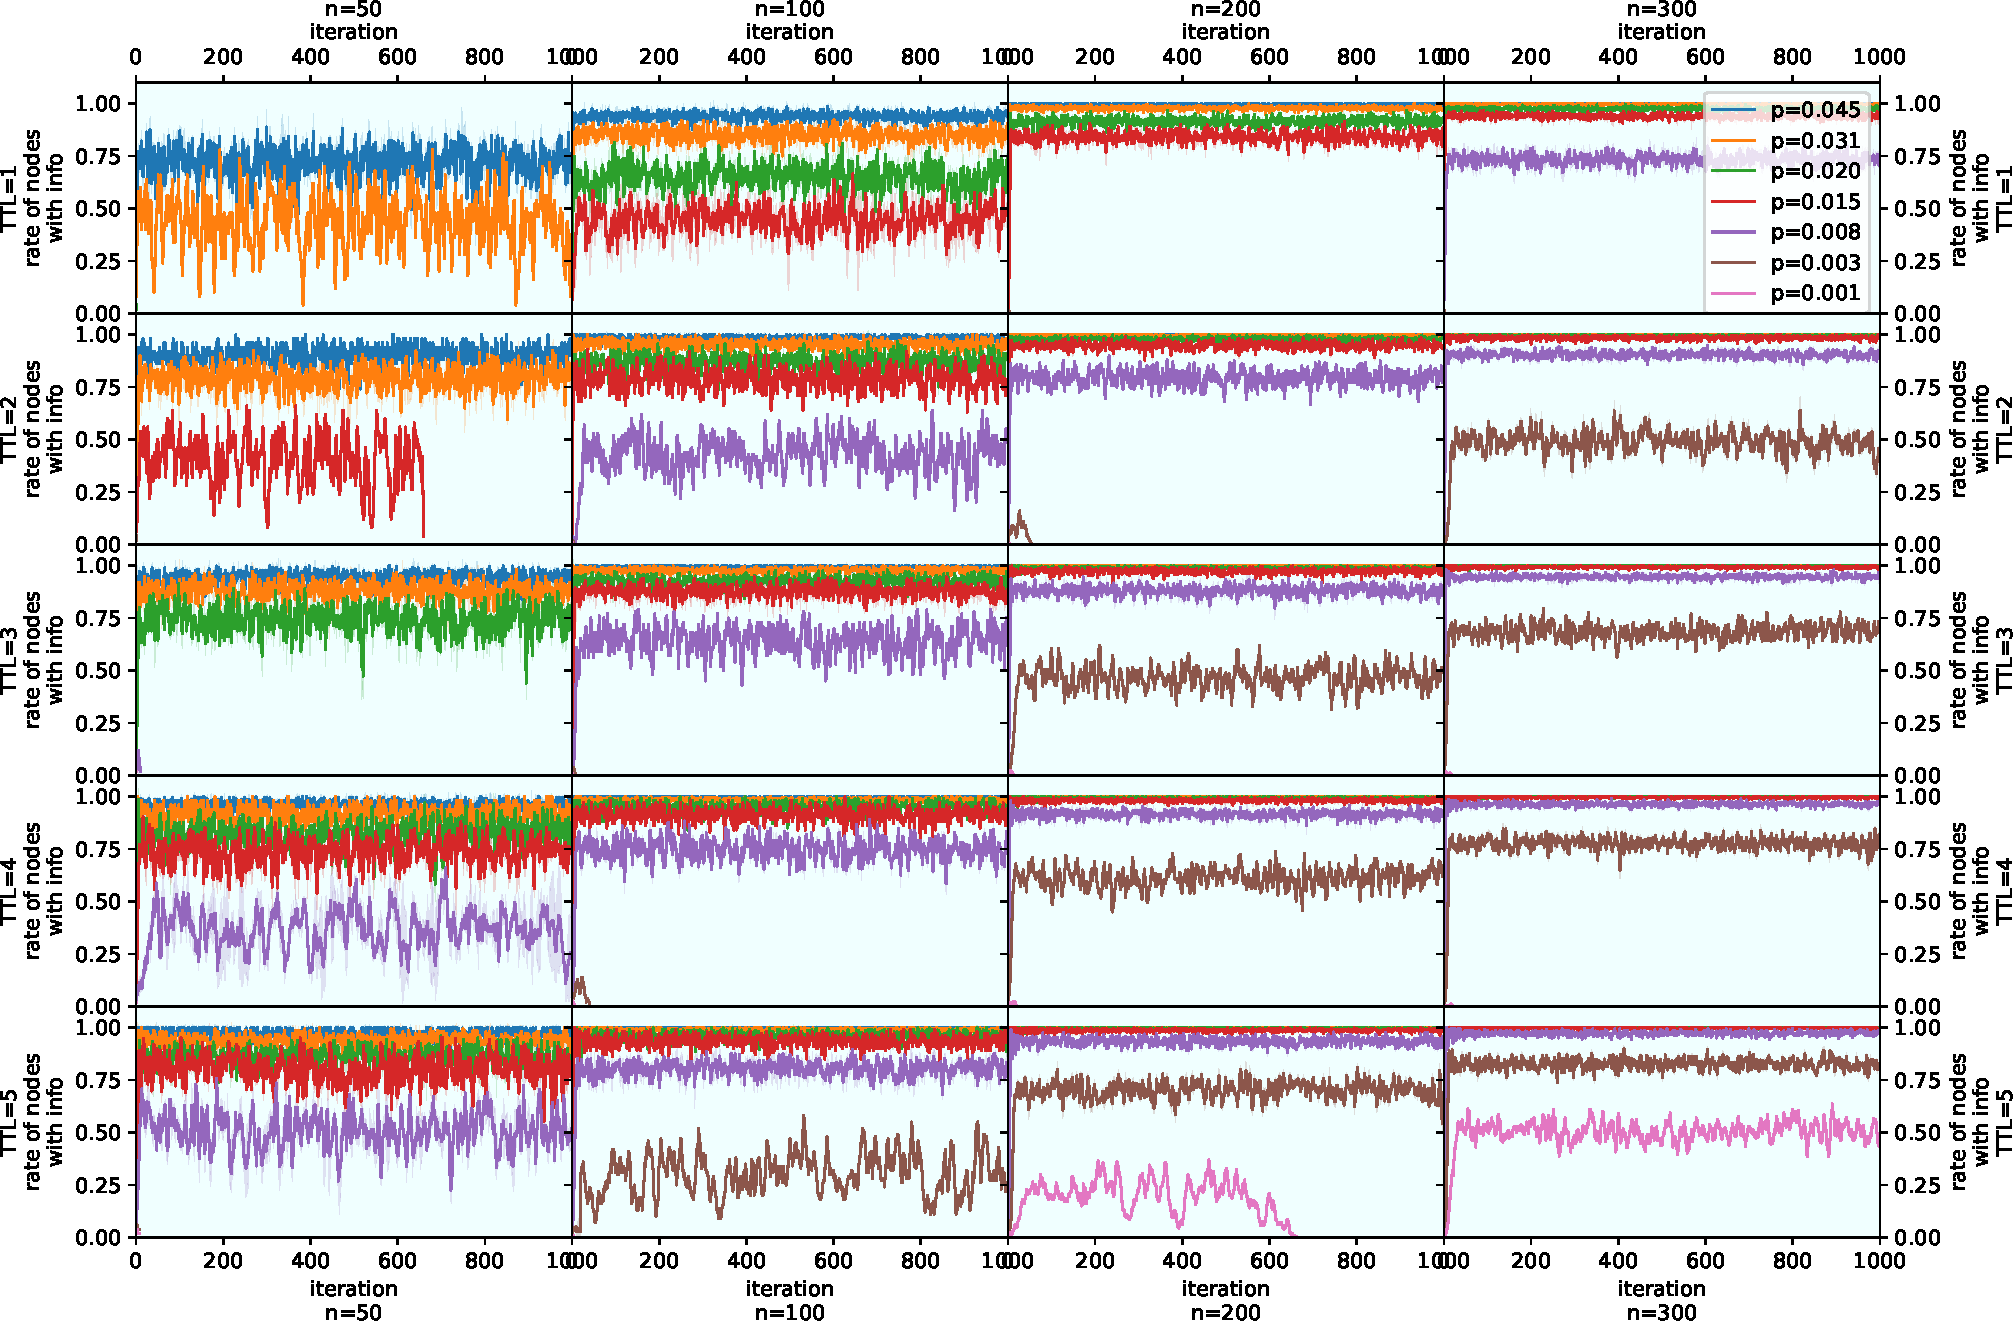
\includegraphics[width=1\linewidth]{results/frac_info_edge}
	\caption{Fraction of the nodes with information in Edge Markovian model dynamic graph. Time traces were averaged over 15 experiments. The color area around curves is their respective standard deviation.}
	\label{fig:fracinfoedge}
\end{sidewaysfigure}


Clearly, with higher $n$ and higher $d$, the information has more chances to persist up to \nth{100} iteration, as shown in Fig~\ref{fig:succrate}. The Manhattan model seems to have the best performance in preserving information in unfavorable conditions -- low TTL and low $d$. However, when condition for the information persistence are relatively good -- $TTL \geq 4$ and $d$ -- the Edge Markovian graph preserves the message with 100\% yield. Additionally, the figure depicts the gradual transition between the conditions not preserving the message and providing 100\% message persistence. In the case of the Edge Markovian model, the dependence of the success of preserving the message on $n$ and $p$ is very sharp for all values of TTL.

\begin{figure}[!h]
	\centering
	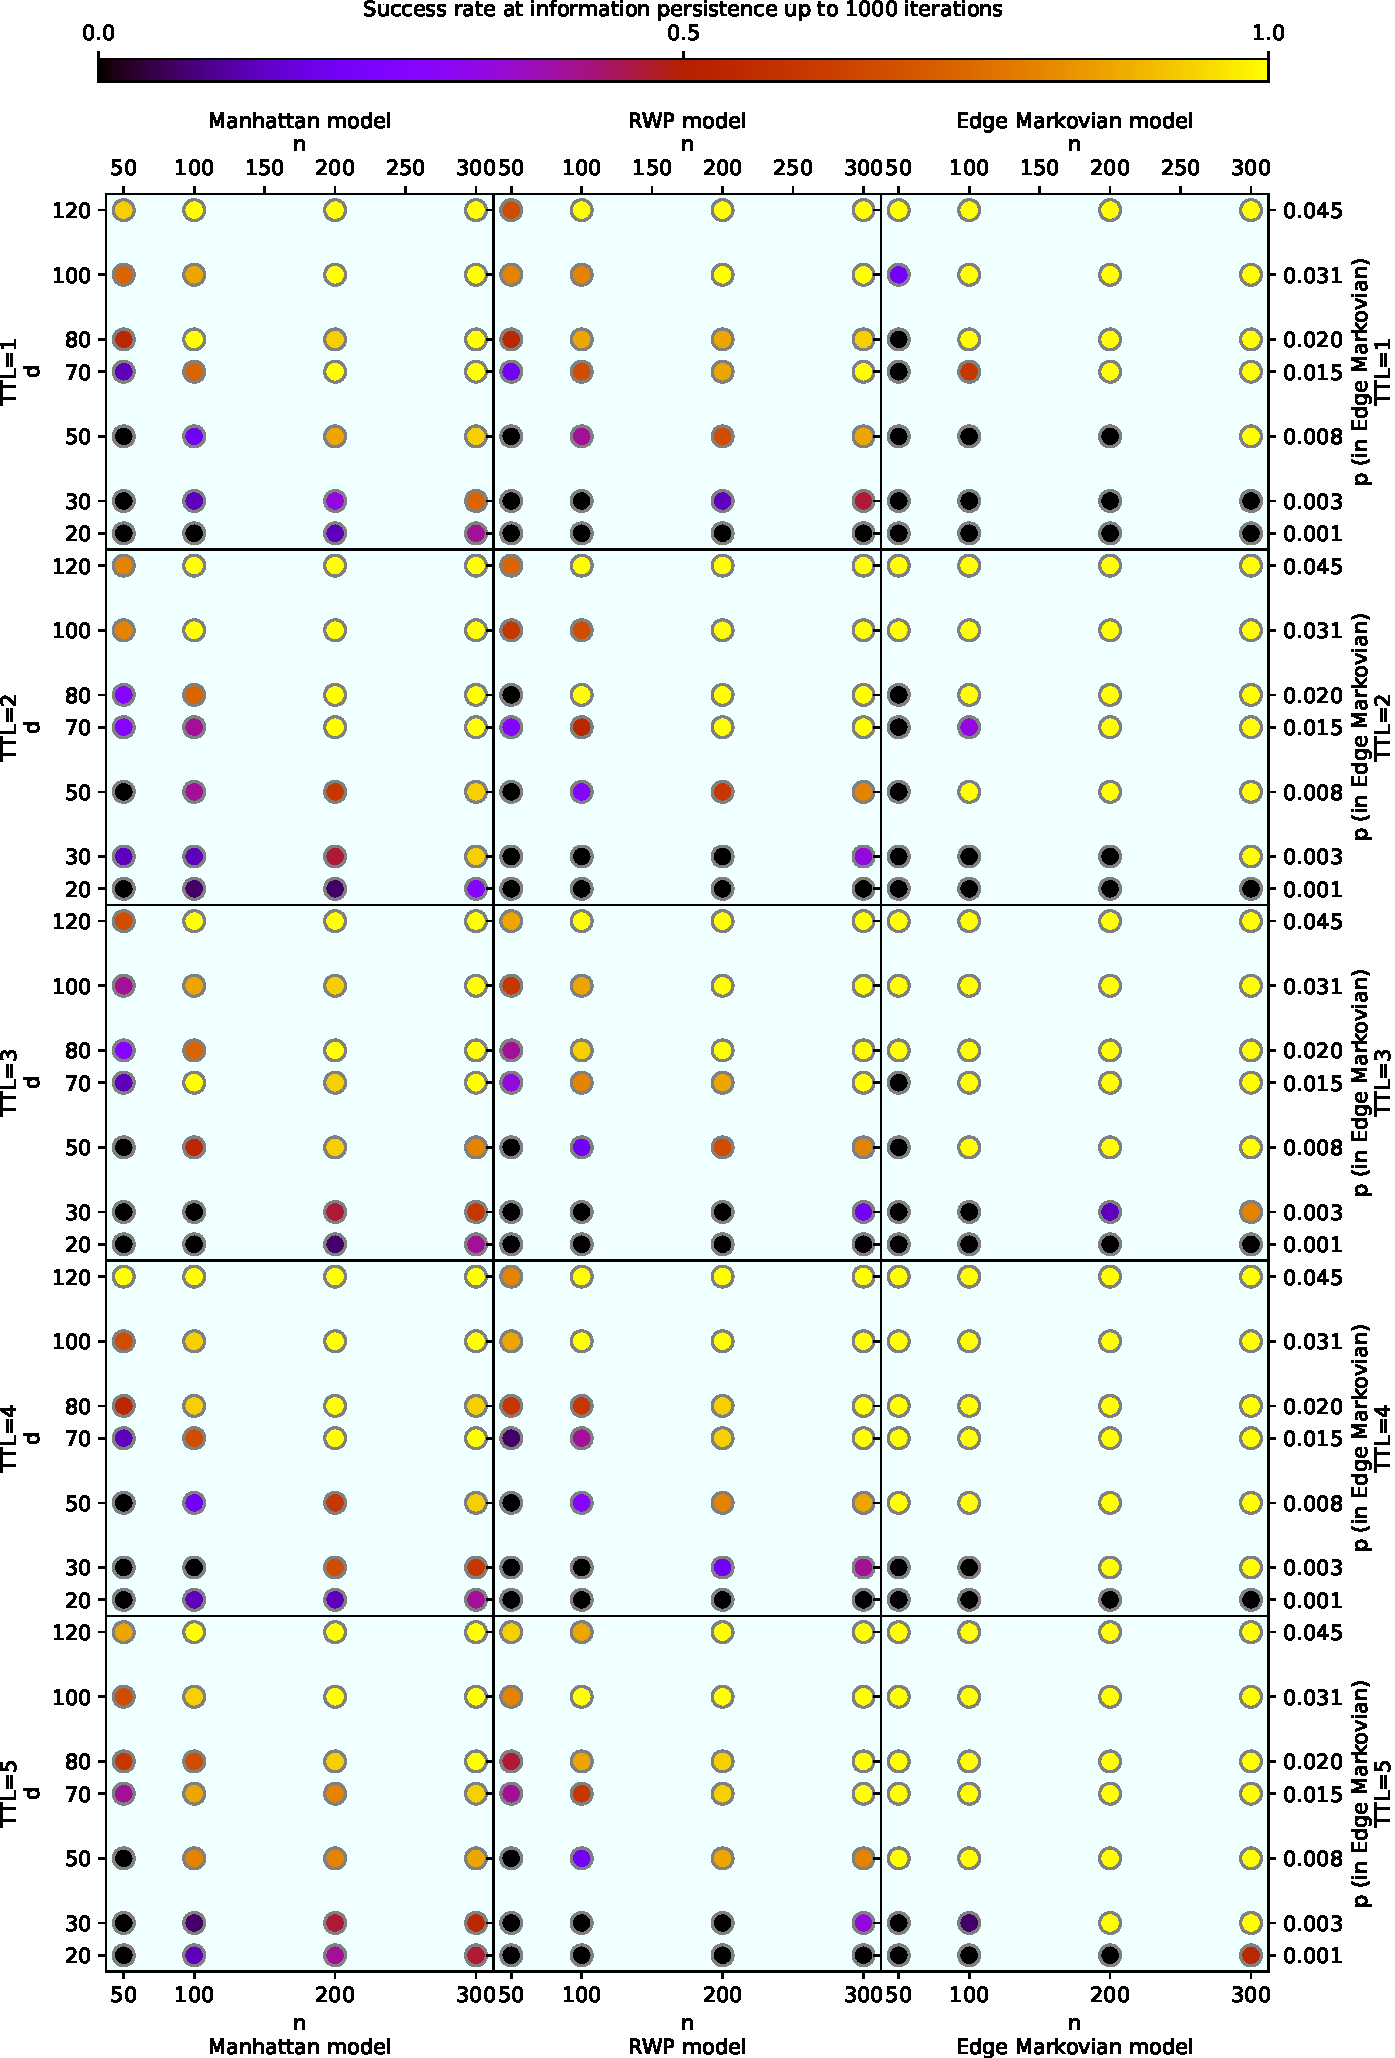
\includegraphics[width=0.95\linewidth]{results/succ_rate}
	\caption{Fraction of the experiments (out of 15 total) where information survived up to \nth{1000} iteration.}
	\label{fig:succrate}
\end{figure}




\clearpage
\bibliographystyle{plJAmChemSoc_all}
\bibliography{information_persistance}



\end{document}